\documentclass[tikz, border=5pt]{standalone}

% Required packages
\usepackage{pgfplots}
\usepackage{pgfplotstable}
\usepackage{tikzviolinplots}
\pgfplotsset{compat=1.18}

\usepackage{cite}
\usepackage{amsmath,amssymb,amsfonts}
\usepackage{algorithmic}
\usepackage{graphicx}
\usepackage{textcomp}
\usepackage{xcolor}
\usepackage{tikz}
\usepackage{physics}
\usepackage{algorithm}
\usepackage{pgfplots}
\usepackage{pgfplotstable}
% \usepackage[sorting=none]{biblatex}
\usepgfplotslibrary{statistics}
\usepackage{etoolbox} % for \ifnumcomp
\usepackage{listofitems} % for \readlist to create arrays
% \usepackage[ruled,vlined]{algorithm% Increase row height
\renewcommand{\arraystretch}{1.4}

% Adjust column spacing
\setlength{\tabcolsep}{8pt}  % default is 6pt, increasing it for better spacing

\tikzset{>=latex} % for LaTeX arrow head
\colorlet{myred}{red!80!black}
\colorlet{myblue}{blue!80!black}
\colorlet{mygreen}{green!60!black}
\colorlet{mydarkred}{myred!40!black}
\colorlet{mydarkblue}{myblue!40!black}
\colorlet{mydarkgreen}{mygreen!40!black}
\tikzstyle{node}=[very thick,circle,draw=myblue,minimum size=22,inner sep=0.5,outer sep=0.6]
\tikzstyle{connect}=[->,thick,mydarkblue,shorten >=1]
\tikzset{ % node styles, numbered for easy mapping with \nstyle
  node 1/.style={node,mydarkgreen,draw=mygreen,fill=mygreen!25},
  node 2/.style={node,mydarkblue,draw=myblue,fill=myblue!20},
  node 3/.style={node,mydarkred,draw=myred,fill=myred!20},
}
\def\nstyle{int(\lay<\Nnodlen?min(2,\lay):3)} % map layer number onto 1, 2, or 3

\usetikzlibrary{arrows.meta,shadows,positioning}
\usetikzlibrary{calc}
\usetikzlibrary{fit, positioning, shapes.geometric}
\tikzset{
	frame/.style={
		rectangle, draw,
		text width=6em, text centered,
		minimum height=4em,drop shadow,fill=white,
		rounded corners,
	},
	line/.style={
		draw, -{Latex},rounded corners=3mm,
	}
}
% Tikz Library
\usetikzlibrary{calc, quotes, angles}
\pgfmathsetmacro{\r}{0.8}
\pgfmathsetmacro{\Phi}{-160}
\pgfmathsetmacro{\Theta}{-90}
\usepackage{fontawesome5}
\usepackage{float}
% \def\BibTeX{{\rm B\kern-.05em{\sc i\kern-.025em b}\kern-.08em
%     T\kern-.1667em\lower.7ex\hbox{E}\kern-.125emX}}








    \begin{document}

% \begin{figure}[H]
% 	\centering
\begin{tikzpicture}
	% Coordinates
	\coordinate (earth) at (1,2);
	\coordinate (moon) at (8,1);
	\coordinate (earth-point1) at ({\r*cos(\Theta)+1},{\r*sin(\Theta)+2});
	\coordinate (A) at (-.5,.5);
	\coordinate (B) at (8.5,-0.5);
	
	% Earth
	\draw[thick, fill=black!30, draw=black!30
	] (earth) circle (\r);
	\node[inner sep=0pt] (Earth_c) at (earth) {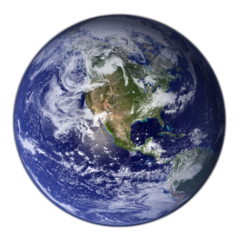
\includegraphics[width=1.8cm]{../../Figure/TBP/Earth.png}};
	% Text
	\node[below, shift={(0,-0.8)}] at (earth) {$m_1$};
	\node (a) at (A) {Earth};
	
	% Moon
	\node[circle, inner sep=5.5pt, fill=black!30] (MOON) at (moon) {};
	\node[inner sep=0pt] (moon_c) at (moon) {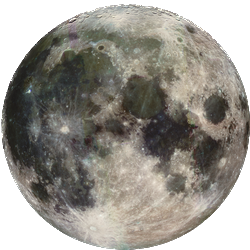
\includegraphics[width=.5cm]{../../Figure/TBP/Moon.png}};
	% Text 
	\node[below, shift={(0,-0.4)}] at (MOON) {$m_2$};
	\node (b) at (B) {Moon};
	
	% Lines
	\draw[-stealth] (a) to[bend left=30] ({\r*cos(\Phi)+1},{\r*sin(\Phi)+2});
	\draw[-stealth] (b) to[bend left=-30] (MOON);
	\draw[dashed, black] (earth) -- (MOON.center);
	
	% center of mass 0.25 from earth
	\coordinate (center) at ($(earth)!0.3!(MOON)$);
	% small circle
	\draw[fill=black] (center) circle (1.5pt) node[below, shift={(0,-0.1)}] {Center of Mass};
	
	% Calculate direction from Earth to Moon
	\pgfmathsetmacro{\xDiff}{8 - 1} % X difference between Moon and Earth
	\pgfmathsetmacro{\yDiff}{1 - 2} % Y difference between Moon and Earth
	\pgfmathsetmacro{\angle}{atan2(\yDiff,\xDiff)} % Angle of the line
	
	% Add axes at center of mass
	\draw[->, thick] (center) -- ++(\angle:2) node[above, shift={(0,0.2)}] {X-axis};
	\draw[->, thick] (center) -- ++(\angle+90:2) node[above] {Y-axis};
	
	% add satellite with shift
	\coordinate (satellite) at ($(center)!0.5!(MOON)+(0,2)$);
	\node (satellite) at (satellite) {\faSatellite};
	
	% connect earth to satellite r1
	\draw[-stealth] (earth) -- (satellite) node[pos=0.3, above] {$\vb{r}_1$};   
	% connect moon to satellite r2
	\draw[-stealth] (MOON) -- (satellite) node[pos=0.5, above] {$\vb{r}_2$};
	% connect center of mass to satellite r
	\draw[-stealth] (center) -- (satellite) node[pos=0.5, above] {$\vb{r}$};
	% add line to show satellite is in between
	\node (c) at ($(satellite)+(1.5,0.5)$) {Satellite};
	\draw[-stealth] (c) to[bend left=30] (satellite);
	
\end{tikzpicture}
%   \caption{Neural network architecture of the actor in the DDPG algorithm.}
%   \label{fig:actor_nn}
% \end{figure}


\end{document}